
\chapter{Analýza požadavků}\label{kap:pozadavky}

V této kapitole budou popsány požadavky na aplikaci, ke kterým jsme dospěli na základě diskuze s vedoucím a analýzy existujících řešení. Požadavky jsou poté sdruženy do případů užití, podle kterých je později, v kapitole \ref{kap:navrh} proveden návrh aplikace.  

\section{Uživatelské role}\label{sec:role}

V této sekci popíšeme role, které mají předpokládaní uživatelé aplikace. Od těchto rolí následně odvodíme jejích požadavky. Uživatelské role a požadavky jsou formulovány na základě představy o zástupcích těchto rolí a jejich potřebách.

Uživatele aplikace můžeme rozdělit do 3 hlavních skupin --- zájemci ze široké veřejnosti, poskytovatelé dat a novináři.

\subsection{Role: veřejnost}

První skupinou uživatelů aplikace jsou zájemci ze široké veřejnosti. Tato skupina má zájem prohlížet zveřejněné úřední desky a informace na nich. Je pro ně důležitý obsah informací a jejich aktuálnost. 

Může se jednat například o obyvatele obce, který si chce prohlédnout úřední desku svojí obce a zjistit aktuální informace, které jsou na ní vyvěšené (např. uzavření komunikace nebo odstávka elektřiny). Pro takového uživatele je důležité mít možnost rychle vyhledat konkrétní desku a najít mezi informacemi na ní ty aktuální.

Dalším požadavkem z této skupiny uživatelů je vyhledat informace, týkající se podobné tématiky (např. vyhledat pozemky k dražbě). Pro splnění tohoto požadavku je nutné vyhledávání v informacích pomocí klíčových slov.

Uživatel může také potřebovat filtrovat úřední desky podle typu poskytovatele (např. zjistit, které krajské úřady zveřejňují své úřední desky). K rozdělení poskytovatelů do kategorií je možné použít právní formu poskytovatele.

Výše zmíněné příklady uživatelů můžeme označit za IT laiky. Z toho vyplývá, že mají tito uživatelé potřebu, aby byla aplikace vizuálně přehledná a uživatelské rozhraní jednoduché a intuitivní.

\subsection{Role: poskytovatel dat}

Druhou skupinu tvoří uživatelé, kteří jsou napojeni na poskytovatele dat z úředních desek. Tato role rozšiřuje roli veřejnost. Obsahuje tedy všechny požadavky na prohlížení úředních desek a navíc některé speciální požadavky.

Poskytovatelé dat mají zájem o validaci zveřejněných dat, aby si mohli potvrdit, že jsou data v souladu se specifikací OFN a je možné jimi zveřejněná data používat. Poskytovatele zajímají konkrétní technické detaily, které se týkají distribuce jejich úřední desky a její validace.

Tito uživatelé mohou se chtít opakovaně vracet na stránky s vizualizací svojí úřední desky a s výsledky validace. Pro tyto účely je nutné, aby byla možnost se v aplikaci odkázat na detail konkrétní desky pomocí URL.

\subsection{Role: novinář}

Poslední skupinu uživatelů tvoří osoby, které mají zájem zjistit kvalitu zveřejněných dat a statistiky které se dat týkají. Tato skupina nepotřebuje znát konkrétní detaily, ale celkový přehled validace dat a statistiku poskytovatelů dat.

\section{Požadavky}

V této části představíme uživatelské požadavky na aplikaci, rozdělené do skupin na základě uživatelských rolí.

\subsection{Požadavky: veřejnost}

Následují požadavky uživatelů s rolí veřejnost.

   \textbf{V01} Aplikace umí zobrazit přehled všech úředních desek, které jsou zveřejněné v NKOD jako otevřená data podle OFN pro úřední desky.
   
    \textbf{V02} V aplikaci je možné vyhledat konkrétní úřední desku podle názvu poskytovatele nebo názvu desky.
    
    \textbf{V03} Úřední desky je možné filtrovat do kategorií na základě právní formy poskytovatele.
    
    \textbf{V04} V aplikaci je možné zobrazit metadata informací, které jsou zveřejněné na konkrétní úřední desce. Aplikace zobrazuje pro každou informaci název, datum vyvěšení, datum relevance, URL stránky, kde je informace zveřejněná a odkazy na přílohy, pokud je informace má.
    
    \textbf{V05} Informace z jedné úřední desky se zobrazují chronologicky od aktuálních ke starším.
    
    \textbf{V06} Mezi informacemi na úřední desce je možné vyhledávat pomocí klíčových slov obsažených v názvu informace.
    
    \textbf{V07} Aplikace umí zobrazit úřední desky na mapě. Uživatel může vyhledat konkrétní úřední desku v mapě ze znalosti lokace poskytovatele desky.

\subsection{Požadavky: poskytovatel dat}

Následují požadavky uživatelů s rolí poskytovatel dat.

    \textbf{P01} V aplikaci je možné přistoupit k vizualizaci konkrétní úřední desky zveřejněné v NKOD podle OFN pro úřední desky na základě IRI distribuce. 

    \textbf{P02} V aplikaci je možné zobrazit validaci dat z úřední desky podle schématu OFN pro úřední desky.

    \textbf{P03} Validace kontroluje, že distribuce úřední desky obsahuje všechny doporučené atributy podle minimalistického příkladu dat v OFN pro úřední desky. Aplikace zobrazí uživateli chybějící doporučené atributy.
    
    \textbf{P04} Výsledek validace úřední desky (validní / nevalidní) je zobrazen takovým způsobem, aby byl uživateli zřejmý.
    
    \textbf{P05} Aplikace upozorní uživatele, pokud distribuci desky není možné stáhnout a nabídne možná řešení.
    
    \textbf{P06} Aplikace umožní vyhledat výsledky validace konkrétní úřední desky podle názvu poskytovatele.
    
    \textbf{P07} Výsledky validace úředních desek je možné filtrovat do kategorií na základě právní formy poskytovatele.
    
\subsection{Požadavky: novinář}

Následují požadavky uživatelů s rolí novinář.

    \textbf{N01} Aplikace umí zobrazit statistiku poskytovatelů dat podle právní formy, tedy jaká část z existujících orgánů dané právní formy poskytuje svoji úřední desku jako otevřená data.
    
    \textbf{N02} Aplikace umí zobrazit shrnutí výsledků validace všech úředních desek. Patří sem podíl distribucí desek, které není možné stáhnout, a podíl desek, kterým chybí některé doporučené parametry, ze všech desek.

\subsection{Technické požadavky}\label{sub:tech-poz}

Po konzultaci s vedoucím vznikly další technické požadavky na implementaci a nasazení aplikace.

    \textbf{T01} Aplikace je nasazená pomocí služby GitHub Pages \footnote{\url{https://docs.github.com/en/pages/getting-started-with-github-pages}}.
    
Pro aplikaci jsme chtěli najít řešení pro nasazení a hosting, u kterého by nebylo potřeba udržovat server s veřejnou IP adresou. Jako takové řešení jsme vybrali službu GitHub Pages.

\section{Případy užití} \label{sec:use-cases}

Tato část je věnovaná případům užití aplikace. Při analýze požadavků jsme identifikovali následující případy užití:
\begin{enumerate}
    \item \textbf{UC1} Přehled poskytování dat právními formami. \autoref{use-case:who}
    \item \textbf{UC2} Zobrazení aktuálních informací určité tématiky z konkrétní úřední desky. \autoref{use-case:info}
    \item \textbf{UC3} Vyhledání úřední desky ze znalosti geografické polohy poskytovatele. \autoref{use-case:mapa}
    \item \textbf{UC4} Ověření korektního poskytování dat. \autoref{use-case:validace}
    \item \textbf{UC5} Zjištění stavu poskytovaných dat v rámci právní formy. \autoref{use-case:statAVal}
    \item \textbf{UC6} Zjištění celkové kvality poskytovaných dat. \autoref{use-case:celaVal}
\end{enumerate}

\begin{figure} 
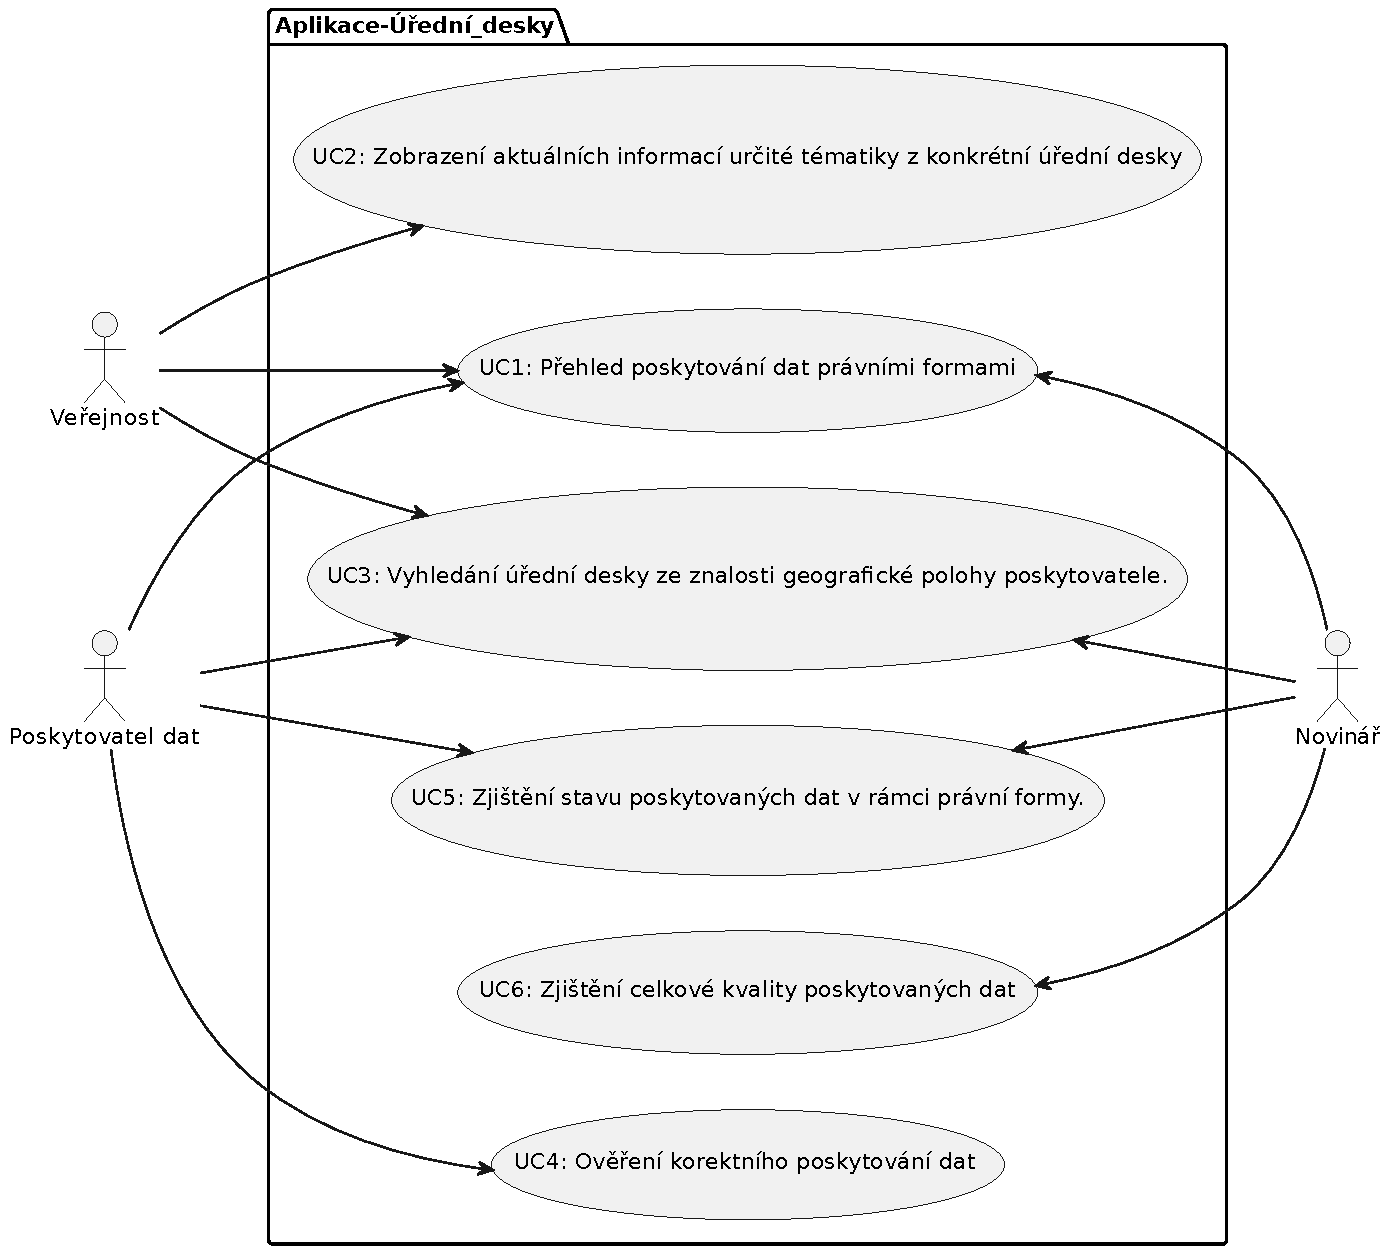
\includegraphics[width=\textwidth]{cs/obrazky/use-case-diagram.pdf}
\caption{Diagram případů užití}
\label{fig:use-case}
\end{figure}

Na obrázku \ref{fig:use-case} můžeme vidět diagram případů užití. Dále podrobně popíšeme jednotlivé případy užití.

%%%%%%%%%%%%%%%%%%%%%%%%%%%%%%%%%%%%%%%%%%%%%%%%%%%%%%%%%%%%%%

\subsection{Přehled poskytování dat právními formami}
\label{use-case:who}

Uživatel potřebuje zjistit, které orgány určité právní formy poskytují svoji úřední desku jako otevřená data. Například, které krajské úřady poskytují svoji desku.

Pokrývá požadavky: \textbf{V01}, \textbf{V03}

Role: veřejnost, poskytovatel dat, novinář

\paragraph{Počáteční stav} 
Uživatel má v aplikaci otevřený seznam úředních desek. Jsou zobrazené všechny úřední desky, které má aplikace k dispozici.

\paragraph{Normální průběh}
\begin{enumerate}
    \item Uživatel v části s filtrováním podle právních forem nechá vybranou pouze tu právní formu, která ho zajímá.
    \item Aplikace vyfiltruje pouze desky, jejichž poskytovatel má vybranou právní formu.
    \item Uživatel si prohlédne vyfiltrované úřední desky a zjistí, kteří poskytovatelé tam jsou.
\end{enumerate}

\paragraph{Odklonění od normálního průběhu}
\begin{itemize}
    \item Žádný z poskytovatelů úředních desek nemá vybranou právní formu. Aplikace zobrazí po filtrování prázdný seznam.
\end{itemize}

\paragraph{Stav po dokončení}
Uživatel zjistil, které orgány určité právní formy poskytují svoji úřední desku jako otevřená data.

%%%%%%%%%%%%%%%%%%%%%%%%%%%%%%%%%%%%%%%%%%%%%%%%%%%%%%%%%%%%%%

\subsection{Zobrazení aktuálních informací určité tématiky z konkrétní úřední desky}
\label{use-case:info}

Uživatel má zájem prohlédnout si aktuální informace, které se týkají nějakého tématu, z určité úřední desky. Může se například jednat o dražby pozemků v nějaké obci.

Pokrývá požadavky: \textbf{V02}, \textbf{V04}, \textbf{V05}, \textbf{V06}

Role: veřejnost

\paragraph{Počáteční stav} 
Uživatel má v aplikaci otevřený seznam úředních desek. Jsou zobrazené všechny úřední desky, které má aplikace k dispozici.

\paragraph{Normální průběh}
\begin{enumerate}
    \item Uživatel zadá do vyhledávání název poskytovatele úřední desky, kterou chce zobrazit. A stiskne tlačítko \texttt{Najít}.
    \item Aplikace ze všech desek vybere pouze ty, které mají hledaného poskytovatele a zobrazí je.
    \item Uživatel si vybere úřední desku, o kterou má zájem, a stiskne tlačítko \texttt{Zobrazit informace}.
    \item Aplikace získá IRI datové sady vybrané úřední desky a požadavkem do NKOD zjistí URL distribuce datové sady.
    \item Aplikace stáhne distribuci a na základě ní vizualizuje detail desky, přičemž seřadí informace od aktuálních ke starším.
    \item Uživatel zadá klíčové slovo z tématiky informace, kterou chce vyhledat (např. dražba), do vyhledávače a stiskne tlačítko \texttt{Najít}.
    \item Aplikace vyfiltruje pouze ty informace, jejichž název obsahuje dané klíčové slovo.
\end{enumerate}

\paragraph{Odklonění od normálního průběhu}
\begin{itemize}
    \item Daný poskytovatel neposkytuje svoji úřední desku jako otevřená data. Des\-ka se tedy nezobrazí při vyhledávání.
    \item Distribuci desky nelze stáhnout. Aplikace upozorní uživatele, nabídne možnost validovat desku.
    \item Úřední deska neobsahuje informace s danou tématikou. Aplikace po filtrování nezobrazí žádné informace.
\end{itemize}

\paragraph{Stav po dokončení}
Aplikace zobrazuje informace s danou tématikou z určité úřední desky.

%%%%%%%%%%%%%%%%%%%%%%%%%%%%%%%%%%%%%%%%%%%%%%%%%%%%%%%%%%%%%%

\subsection{Vyhledání úřední desky ze znalosti geografické polohy poskytovatele}
\label{use-case:mapa}

Uživatel zná geografickou polohu nějakého poskytovatele a chce najít jeho úřední desku z mapy.

Pokrývá požadavky: \textbf{V01}, \textbf{V07}

Role: veřejnost, poskytovatel dat, novinář

\paragraph{Počáteční stav} 
Uživatel má v aplikaci otevřenou mapu úředních desek. Jsou zobrazené všechny úřední desky, které má aplikace k dispozici.

\paragraph{Normální průběh}
\begin{enumerate}
    \item Uživatel na mapě vyhledá polohu poskytovatele.
    \item Uživatel vybere bod na mapě znázorňující poskytovatele, který ho zajímá a klikne na něj.
    \item Aplikace zobrazí úřední desky vybraného poskytovatele.
    \item Uživatel najde mezi zobrazenými úředními deskami tu, která ho zajímá.
\end{enumerate}

\paragraph{Odklonění od normálního průběhu}
\begin{itemize}
    \item Daný poskytovatel neposkytuje svoji úřední desku jako otevřená data. V mapě se nezobrazí bod s poskytovatelem.
\end{itemize}

\paragraph{Stav po dokončení}
Uživatel našel úřední desku v mapě podle polohy poskytovatele.

\subsection{Ověření korektního poskytování dat} \label{use-case:validace}

Uživatel v roli poskytovatele dat chce ověřit, že data z jeho úřední desky jsou zveřejněná, je možné s nimi pracovat a odpovídají specifikaci OFN pro úřední desky.

Pokrývá požadavky: \textbf{P01}, \textbf{P02}, \textbf{P03}, \textbf{P04}, \textbf{P05}, \textbf{P06}

Role: poskytovatel dat

\paragraph{Počáteční stav} 
Uživatel má v NKOD zveřejněná data z úřední desky jako otevřená data a chce provést aktualizaci datové sady. Uživatel už s aplikací pracoval a má k dispozici URL detailu svojí úřední desky, které je vytvořené z IRI datové sady v NKOD. Uživatel aktualizuje data.

\paragraph{Normální průběh}
\begin{enumerate}
    \item Uživatel otevře URL vizualizace detailu svojí úřední desky.
    \item Aplikace zobrazí vizualizaci desky.
    \item Uživatel ověří, že deska obsahuje aktualizované informace.
    \item Uživatel přejde na validační detail desky. Buď využije tlačítka \texttt{Validovat desku} ve vizualizaci, nebo přejde do sekce Validace, vyhledá desku v seznamu výsledků validace a přejde do detailu.
    \item Aplikace provede validaci a zobrazí výsledky. 
    \item Aplikace barevně zvýrazní výsledek --- zelená: validace je v pořádku, žlutá: chybí doporučené atributy, červená: nelze stáhnout distribuci.
    \item Aplikace zobrazí detaily validace --- případné chybějící atributy, nebo chybovou hlášku získanou při stahování distribuce a možné příčiny chyby.
    \item Uživatel zjistí výsledek validace svých dat.
\end{enumerate}

\paragraph{Odklonění od normálního průběhu}
\begin{itemize}
    \item Aktualizace dat změnila datovou sadu tak, že ji není možné aplikací vyhledat v NKOD (případně URL uživatele je poškozené). Aplikace zobrazí chybovou hlášku.
\end{itemize}

\paragraph{Stav po dokončení}
Uživatel ověřil, že jsou aktualizovaná data validně zveřejněná.

\subsection{Zjištění stavu poskytovaných dat v rámci právní formy} \label{use-case:statAVal}

Uživatel chce zjistit, kolik organizací nějaké právní formy poskytuje svoji úřední desku jako otevřená data a jaká je kvalita těchto dat.

Pokrývá požadavky: \textbf{P02}, \textbf{P03}, \textbf{P04}, \textbf{P07}, \textbf{N01}  

Role: poskytovatel dat, novinář

\paragraph{Počáteční stav} 
Uživatel má v aplikaci otevřenou sekci se statistikou poskytovatelů.

\paragraph{Normální průběh}
\begin{enumerate}
    \item Aplikace zobrazí pro vybrané právní formy (obsahující největší skupiny poskytovatelů) na základě dat z RPP kolik je v dané právní formě celkem organizací a kolik z nich poskytují svoji úřední desku jako otevřená data.
    \item Uživatel najde mezi právními formami tu, která ho zajímá a zjistí, jaká část organizací poskytuje svoji úřední desku.
    \item Uživatel přejde do části validace dat.
    \item Aplikace zobrazí seznam stručných výsledků validace pro všechny úřední desky.
    \item Uživatel v části s filtrováním podle právních forem nechá vybranou pouze tu právní formu, která ho zajímá.
    \item Aplikace vyfiltruje pouze výsledky validace desek, jejichž poskytovatel má vybranou právní formu.
    \item Uživatel si prohlédne výsledky validace pro vybranou kategorii.
\end{enumerate}

\paragraph{Odklonění od normálního průběhu}
\begin{itemize}
    \item V uživatelem vybrané právní formě nejsou žádní poskytovatelé dat z úředních desek. Uživatel zjistí pouze celkový počet organizací této právní formy.
\end{itemize}

\paragraph{Stav po dokončení}
Uživatel zjistil stav poskytovaných dat v rámci vybrané právní formy.

\subsection{Zjištění celkové kvality poskytovaných dat} \label{use-case:celaVal}

Uživatel chce zjistit souhrnnou kvalitu otevřených dat z úředních desek.

Pokrývá požadavky: \textbf{P02}, \textbf{P03}, \textbf{N02}  

Role: novinář

\paragraph{Počáteční stav} 
Uživatel má v aplikaci otevřenou sekci se statistikou validace.

\paragraph{Normální průběh}
\begin{enumerate}
    \item Aplikace zobrazí provede validaci všech distribucí úředních desek.
    \item Aplikace zobrazí uživateli následující údaje: kolik distribucí se podařilo (nepodařilo) stáhnout, kolika distribucím chybí některé doporučené atributy. Výsledky zobrazí v textové podobě a procentuálně na koláčovém grafu.
    \item Uživatel si prohlédne souhrnné výsledky validace.
\end{enumerate}

\paragraph{Stav po dokončení}
Uživatel zjistil souhrnnou kvalitu otevřených dat z úředních desek.

